\section{Theoretische Grundlagen}

Bei einem stabilen Atom ist das Verhältnis zwischen der Neutronen und Protonenanzahl im Kern meist in engen Grenzen.
Wenn das Verhältnis der beiden Teilchen diese Grenze allerdings überschreitet wird der vorliegende Atomkern instabil und er zerfällt in 
unterschiedlichen Zerfallsprozessen in ein stabiles Atom. Je nach instabilem Atom und Anzahl der Protonen und Neutronen findet ein anderer
Zerfallsprozess statt.
\\
\newline
Eine wichtige zu betrachtende Größe in der Kernphysik ist die Halbwertszeit $T$, sie entspricht dem Zeitraum $\increment t$ in der eine Anzahl von instabilen
Kernen gerade um die Hälfte zerfallen ist. Die Halbwertszeit instabiler Atomkerne variiert dabei in der Größenordnung 
$t = \SI{10e23}{\second}$, deshalb werden im Folgenden Halbwertszeiten von Atomen betrachtet die im Bereich einiger Sekunden bis Stunden liegen.
Diese Atomkerne müssen vor der Versuchsdurchführung erzeugt werden, dazu wird ein stabiler Atomkern mit einem Neutron beschossen. Die Neutronen haben dabei
den Vorteil ladungsfrei zu sein und somit nicht die Potentialbarriere des Atomkerns überwinden zu müssen.

\subsection{Kernreaktionen mit Neutronen}
Die Wechselwirkung eines Teilchens mit einem Atomkern wird Kernreaktion genannt. 
Unter Verwendung von Neutronen kann dieses Neutron in einen stabilen Atomkern $A$ eindringen und durch die Absorption des Neutrons
entsteht anschließend ein neuer Kern $A^{*}$. In diesem Zustand besitzt der sogenannte Zwischenkern eine Energie welche um die kinetische- und Bindungsenergie
des aufgenommenen Neutrons höher ist, als der vorherige Zustand $A$. Die aufgenommene Energie sorgt für die Anregung vieler Protonen und Neutronen auf höhere Energiezustände
wodurch der Kern $A^{*}$ kein Neutron oder anderes schweres Teilchen mehr abstoßen kann. 
\\
Wenn dies der Fall ist geht der angeregte Zustand $A^{*}$ über folgende Reaktionen wieder in einen stabilen Zustand zurück.
\begin{equation}
    \ce{^{m}_{z}A + ^{1}_{0}\symup{n} -> ^{m+1}_{z}A^{*} -> ^{m+1}_{z}A} + \gamma
\end{equation}
Hier ist $m$ die Massenzahl, also die Anzahl an Neutronen und Protonen, $z$ die Kernladungszahl, also die Anzahl der Protonen und $\gamma$ ist ein durch den Übergang zu dem nicht angeregten Kernzustand $A$
entstehendes hochenergetisches Photon.
\\
Der entstehende Zustand besitzt allerdings immer noch ein zusätzliches Neutron wodurch es weiterhin kein stabiler Atomkern ist. Unter Abgabe eines Elektrons und Antineutrinos entsteht ein stabiler Kern
mit einer erhöhten Kernladungszahl, also mit einem Proton mehr. Diese Umwandlung lässt sich folgendermaßen aufschreiben.
\begin{equation}
\label{eqn:zerfalleinfach}
\ce{^{m+1}_{z}A -> ^{m+1}_{z+1}C} +\beta^{-} + \bar{\nu_{e}} + E_{\text{kin}}
\end{equation}
Das ${\beta}^{-}$ ist dabei der $\beta$-Zerfall bei dem unter Abgabe eines Elektrons und Antineutrinos ein Proton entsteht.
Die zusätzliche kinetische Energie entsteht durch einen Massenunterschied der Zustände vor und nach dem Zerfall und bezieht sich auf das austretende Elektron und Antineutrino. Dieser Effekt wird
Massendefekt genannt und kann über 
\begin{equation}
\label{eqn:einsteineq}
\increment E = \increment m \cdot c^2
\end{equation}
bestimmt werden. 
\\
Wenn ein Atomkern mit einem Neutron beschossen wird, kommt es allerdings nicht immer zu einer Absorption. Die Wahrscheinlichkeit mit der ein Neutron von einem Atomkern eingefangen wird nennt sich
Wirkungsquerschnitt und wird mit $\sigma$ abgekürzt.
Der Wirkungsquerschnitt ist dabei die Fläche die der Kern besitzen müsste, um alle auftreffenden Neutronen einzufangen, er ist definiert als
\begin{equation}
\sigma = \frac{u}{nKd}
\end{equation}
Dabei ist $u$ die Anzahl der Einfänge, $n$ die Anzahl der Neutronen pro Sekunde, $d$ die Dicke der Atome in $\si{\centi\meter\squared}$ und $K$ die Anzahl der Atome in $\si{\centi\meter\cubed}$
Der Wirkungsquerschnitt hängt stark von der Geschwindigkeit der Neutronen ab, dehalb wird zwischen schnellen und langsamen Neutronen unterschieden.
Bei der Betrachtung der De-Broglie Wellenlänge
\begin{equation}
\lambda = \frac{h}{m_{\text{Neutron}} \cdot v} 
\end{equation}
ist zu erkennen, dass bei hohen Geschwindigkeit die Materiewelle deutlich kleiner wird. Hier kann eine geometrische Betrachtung den Wirkungsquerschnitt ersetzen, denn $\lambda << R$ wobei $R$ der Kernradius ist.
Bei kleinen Geschwindigkeiten hingegen sind die geometrischen Überlegungen unbrauchbar und der Wirkungsquerschnitt ist mehrere Zehnerpotenzen größer als die der geometrische Betrachtung.
Die Formel zur Berechnung des Querschnitts berücksichtigt nun die Energiedifferenzen der einzelnen Energieniveaus des Kerns, bei der ein Neutron vom Atomkern absorbiert wird.
Berechnet wird diese durch
\begin{equation}
\sigma(E) = \sigma_{0} \sqrt{\frac{E_{r_{i}}}{E}} \cdot \frac{\tilde{c}}{(E - E_{r_{i}})^{2} + \tilde{c}}
\end{equation}
wobei $\tilde c$ und $\sigma_{0}$ charakteristische Konstanten der Kernreaktion sind. $E_{{r}_{i}}$ sind die Energieniveaus des Zwischenkerns und somit wird für eine Energie $E = E_{{r}_{i}}$
der Wirkungsquerschnitt maximal. Wenn allerdings $E << E_{{r}_{i}}$ ist, dann gilt
\begin{equation}
\sigma \propto \frac{1}{\sqrt{E}} \propto \frac{1}{v}
\end{equation}
somit existiert bei niedrigerer Neutronengeschwindigkeit eine höherer Wirkungsquerschnitt und somit eine höhrere Wahrscheinlichkeit von dem Atomkern aufgenommen zu werden.
In dem Versuch wurden genau diese langsamen Neutronen verwendet und die Erzeugung dieser Neutronen wird im Folgenden diskutiert.

\subsection{Erzeugung niederenergetischer Neutronen}
Ein Neutron als freies Teilchen ist instabil daher muss es für die Verwendung von Kernreaktionen zunächst erzeugt werden.
In diesem Fall wird dies durch einen Beschuss von $\alpha$-Teilchen auf Berylliumkerne ($\ce{^{9}Be}$) erlangt.
Der Zerfallprozess sieht hier folgendermaßen aus.
\begin{equation}
\ce{^{9}_{4}Be + ^{4}_{2}{\alpha} -> ^{12}_{6}C + ^{1}_{0}n}
\end{equation}
Dabei wurden die $\alpha$-Teilchen aus dem Zerfall von $\ce{^{226}Ra}$-Kernen gewonnen. Um diese Neutronen nun abzubremsen werden dicke Materieschichten verwendet durch die sie hindurchdiffundieren müssen.
Diese Materieschichten müssen aus leichten Kernen bestehen, damit die Neutronen möglichst viel Energie an die Materieschicht abgeben. Das liegt an dem allgemeinen Gesetz
des elastischen Stoßes.
\begin{equation}
E_{ü} = E_{0} \cdot \frac{4Mm}{(M+m)^{2}}
\end{equation}
Die übergebene Energie $E_{ü}$ wird also umso größer je näher die beiden Massen $m$ und $M$ aneinander liegen.
Aufgrund dieser Überlegungen eignet sich Wasserstoff besonders gut und die benutzte Neutronenquelle wird deshalb mit Paraffin ummantelt.
Die mittlere kinetische Energie der Neutronen nach einigen Stößen mit der Paraffinschicht beträgt
\begin{equation*}
\overline{E_{\text{kin}}} = \SI{0.025}{\electronvolt} \quad \to \quad \overline{v_{\text{Neutron}}} = \SI{2.2e6}{\meter\per\second}
\end{equation*}
Dies gilt für eine Temperatur von $T = \SI{290}{\kelvin}$. Die Neutronen mit diesen Energien werden thermische Neutronen genannt.

\subsection{Zerfallsgesetz und Bestimmung der Halbwertszeit}
Die zu untersuchenden Zerfälle von Vanadium und Rhodium gehorchen den Gesetzmäßigkeiten des radioaktiven Zerfalles. Dieses besagt, dass die Zählrate $N(t)$ der noch nicht zerfallenen Kerne durch
\begin{equation}
\label{eqn:zerfallsgesetz}
N(t) = N_{0} e^{-\lambda t}
\end{equation}
gegeben ist (siehe \cite{skript2}). $N_{0}$ ist die am Anfang vorliegende Anzahl an instabilen Kernen und $\lambda$ die Zerfallskonstante.
Die Halbwertszeit ist also der Zeitpunkt $t$ bei der $N(t) = 1/2 \, N_{0}$ gilt.
Wenn dies eingesetzt und logarithmiert wird folgt die Halbwertszeit $T$.
\begin{equation}
\label{eqn:187}
\text{ln}\left( \frac{1}{2}\right) = -\lambda T \quad \to \quad T = \frac{\text{ln}(2)}{\lambda}
\end{equation}
Dies führt allerdings in der Durchführung zu Problemen, denn $N(t)$ lässt sich nur unzuverlässig bestimmen, deshalb werden in diesem Versuch die Zerfälle in
festgelegten Zeitintervallen $\increment t$ gemessen.
Die Definition von $N_{\increment t}$ lässt sich nun über das Zerfallsgesetz \eqref{eqn:zerfallsgesetz} schreiben.
\begin{align}
\label{eqn:g1}
N_{\increment t}(t) &=  N(t) - N(t + \increment t) \\
\label{eqn:g2}
N_{\increment t}(t) &= N_{0} (1-e^{-\lambda \increment t}) e^{-\lambda t}
\end{align}
Dabei folgt die Gleichung \eqref{eqn:g2} nach dem Einsetzten von dem Zerfallsgesetz \eqref{eqn:zerfallsgesetz} in Gleichung \eqref{eqn:g1}.
Wird diese Darstellung anschließend logarithmiert, kann ein linearer Zusammenhang festgestellt werden, wodurch sich nachher die Zerfallskonstante $\lambda$ ermitteln lässt.
\begin{equation}
\label{eqn:brrr}
\text{ln}(N_{\increment t}(t)) = \text{ln}(N_{0}(1-e^{-\lambda \increment t})) - \lambda t
\end{equation}
Dabei ist $\text{ln}(N_{0}(1-e^{-\lambda \increment t}))$ der y-Achsenabschnitt und $\lambda$ die gesuchte Steigung.
Problematisch ist hier die Wahl des Zeitintervalls $\increment t$, da es zu großen systematischen oder statistischen Fehlern kommen kann.

\subsection{Zerfall von Vanadium und Rhodium}
Zunächst wird der Zerfall von Vanadium beschrieben, da Rhodium im Vergleich einige Besonderheiten aufweist, auf die eingegangen werden muss.
Wie in dem Zerfallprozess \eqref{eqn:zerfalleinfach} , passiert bei Vanadium $\ce{^{52}_{23}V}$ folgendes.
\begin{equation}
\ce{^{51}_{23}V + ^{1}_{0}n -> ^{52}_{23}V -> ^{52}_{24}Cr} + {\beta}^{-} + \bar{\nu_{e}} 
\end{equation}
Die Besonderheit an Rhodium ($\ce{^{103}_{45}Rh}$) ist, dass bei Beschuss eines Neutrons zwei unterschiedliche instabile Zustände resultieren können. 
Diese sind in den folgenden Zerfallsprozessen angegeben.
\begin{align}
\ce{^{103}_{45}Rh + ^{1}_{0}n &->[10{\si{\percent}}] ^{104\text{i}}_{45}Rh -> ^{104}_{45}Rh} + \gamma \ce{-> ^{104}_{46}Pd} + {\beta}^{-} + \bar{\nu_{e}} \\[3pt]
\ce{^{103}_{45}Rh + ^{1}_{0}n &->[90{\si{\percent}}] ^{104}_{45}Rh -> ^{104}_{46}Pd} + {\beta}^{-} + \bar{\nu_{e}} 
\end{align}
Zu erkennen ist, dass auch ein isomerer Zustand $\ce{^{104{\text{i}}}_{45}Rh}$ auftreteten kann welcher nach einem weiteren Zerfall bei Abgabe eines $\gamma$-Quants wieder zu $\ce{^{104}_{45}Rh}$ wird.
Beide Prozesse laufen allerdings simultan ab und werden beide vom Detektor aufgefasst. 
Die Gesamtaktivität der Probe setzt sich additiv aus den beiden Einzelaktivitäten zusammen. Beide Prozesse besitzen unterschiedliche Halbwertszeiten die hinreichend
groß voneinander abweichen. Nach einiger Zeit ist der Zustand $\ce{^{104}_{45}Rh}$ praktisch zerfallen und nur noch der isomere Zustand $\ce{^104{\text{i}}_{45}Rh}$ mit höherer Halbwertszeit zerfällt.
\\
\newline
Eine solche Zerfallskurve ist in Abbildung \ref{fig:AbbildungKurve} dargestellt.
Zunächst kann an diesem Diagramm ein Zeitpunkt $t^{*}$ abgelesen werden bei dem wieder ein linearer Verlauf entsteht. Nun kann mit Gleichung 
\eqref{eqn:g2} für alle $t_{i} > t_{*}$ eine Gerade mit einem Zerfallskoeffizienten $\lambda_{\text{lang}}$ bestimmt werden.
Für den Zerfall des kurzlebigen Isotops werden von den Gesamtzählraten $N_{\increment t}(t_{i})$ (für $t_{i} < t^{*}$) die Zerfallswerte des langlebigen Isotops abgezogen.
\begin{equation}
N_{{\increment t}_{\text{kurz}}}(t_{i}) = N_{\increment t}(t_{i}) - N_{{\increment t}_{\text{lang}}}(t_{i})
\end{equation}
\\
\begin{flushleft}
$N_{\increment t}(t_{i})$ ergibt sich dabei aus der bereits aufgestellten Gleichung \eqref{eqn:g2} und für $N_{{\increment t}_{\text{lang}}}(t_{i})$ wird diese ebenfalls durch Gleichung \eqref{eqn:g2} zu
\end{flushleft}
\begin{equation}
N_{\increment t_{\text{lang}}}(t) = N_{{0}_{\text{lang}}} (1-e^{-{\lambda}_{\text{lang}} \increment t}) e^{-{\lambda}_{\text{lang}} t}
\end{equation}
\begin{flushleft}
Durch erneute Logarithmierung kann der zugehörige Koeffizient $\lambda_{\text{lang}}$ bestimmt werden. 
\end{flushleft}
\begin{figure}
  \centering
  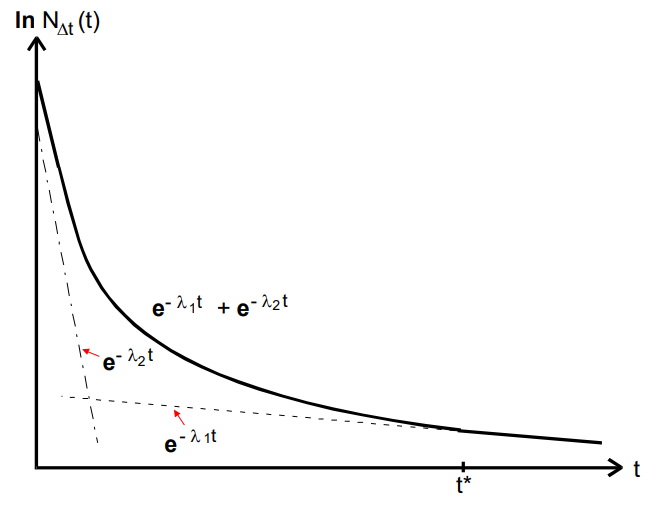
\includegraphics[width=0.7\textwidth]{bilder/AbbildungKurve.png}
  \caption{Zerfallskurve aus 2 Isotopen mit unterschiedlichen Zerfallskonstanten \cite{skript}.}
  \label{fig:AbbildungKurve}
\end{figure}
